\documentclass[11pt, a4paper]{article}
\usepackage[latin1]{inputenc}
\usepackage{pgfplots}
\pgfplotsset{width=\textwidth ,compat=1.9}
\usepackage[dutch]{babel}
\usepackage{csquotes}
\usepackage{amsmath}
\usepackage{amsfonts}
\usepackage{amssymb}
\usepackage[backend=biber, style=numeric, citestyle=numeric-comp, sorting = none]{biblatex}
\author{Stef Tweepenninckx, r0677232}
\title{Practicum 1: Sorteeralgoritmes}


%define printtitle
\makeatletter
\def\printtitle{                 
    {\large \@title}} 
\makeatother

%define printauthor
\makeatletter                       
\def\printauthor{                  
    {\large \@author}}              
\makeatother

\begin{document}
\begin{titlepage}
\newcommand{\HRule}{\rule{\linewidth}{0.5mm}} 
\center 
\textsc{\LARGE Gegevensstructuren en algoritmen}\\[1.5cm] 
\HRule \\[0.4cm]

{\huge \bfseries \printtitle}\\[0.4cm] 
\HRule \\[0.4cm]

\Large \emph{Authors:}\\
 \textsc{\printauthor}\\[3cm]

{\large \textsc{\today}}\\[3cm] 

\vfill 
\end{titlepage}

\section*{Aantal vergelijkingen}
\subsubsection*{Selection sort}
\subsubsection*{Insertion sort}
\subsubsection*{Quicksort}

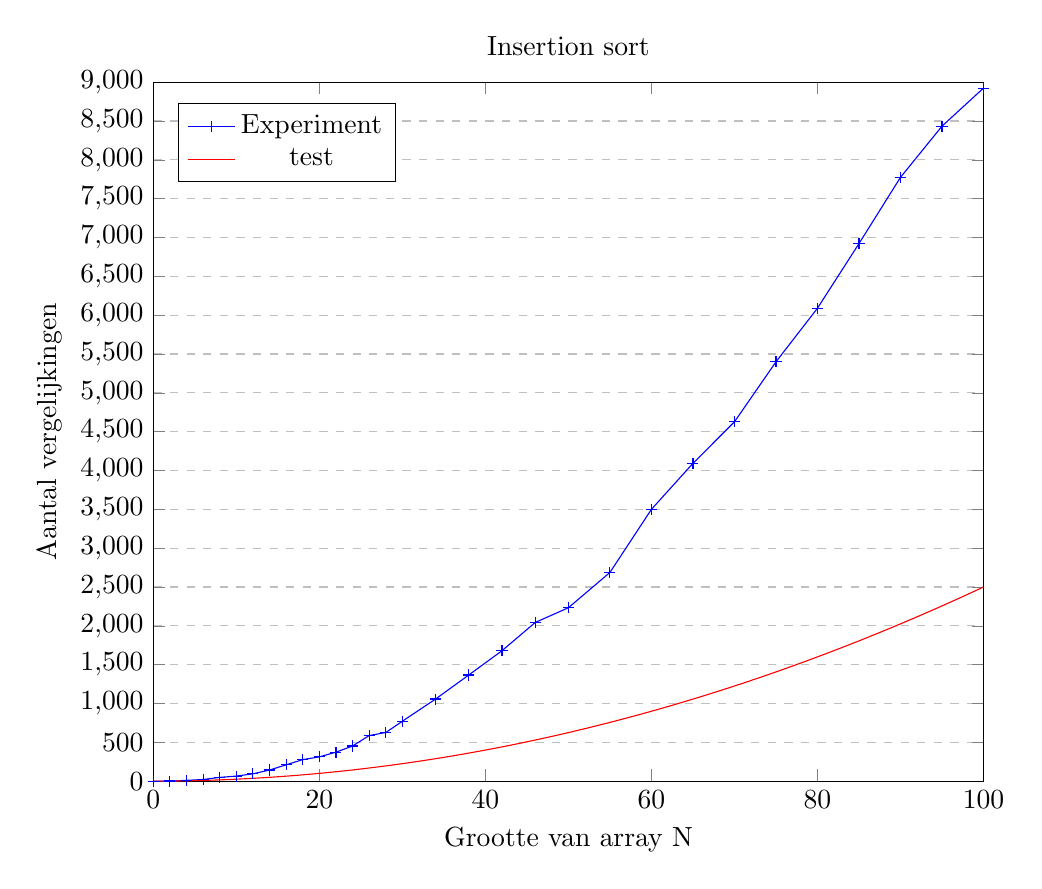
\begin{tikzpicture}
\begin{axis}[
    title={Insertion sort},
    xlabel={Grootte van array N},
    ylabel={Aantal vergelijkingen},
    xmin=0, xmax=100,
    ymin=0, ymax=9000,
    xtick={0,20,40,60,80,100},
    ytick={0,500,1000,1500,2000,2500,3000,3500,4000,4500,5000,5500,6000,6500,7000,7500,8000,8500,9000},
    legend pos=north west,
    ymajorgrids=true,
    grid style=dashed,
]
 
\addplot[
    color=blue,
    mark=+,
    ]
    coordinates {
    (0,0)(2,1)(4,10)(6,21)(8,48)(10,65)(12,94)(14,143)(16,210)(18,277)(20,312)(22,373)(24,452)(26,587)(28,626)(30,771)(34,1057)(38,1367)(42,1679)(46,2043)(50,2233)(55,2687)(60,3500)(65,4092)(70,4627)(75,5399)(80,6090)(85,6922)(90,7775)(95,8434)(100,8924)
    };
    \legend{Experiment};

\addplot [
    domain= 0:100, 
    samples=100, 
    color=red,
    ]
    {(x^2)/4};
    \addlegendentry{test};
	
 
\end{axis}
\end{tikzpicture}
\end{document}